\chapter{Planificación}

\section{Planificación a priori}

Se trata de planificar como se espera desarrollar el proyecto en el tiempo, para ello se va a hacer uso de un diagrama de Gantt donde se va a proporcionar una vista general de las tareas programadas, estas tareas tendrán que completarse en unas fechas estipuladas. Para poder realizar el digrama se tienen que indicar las etapas de desarrollo del proyecto.

\subsection{Etapas de desarrollo}

\begin{itemize}
    \item \textbf{1ª etapa}: Revisar entornos de desarrollo para IoT.
    \item \textbf{2ª etapa}: Desarrollar aplicación para IoT.
    \item \textbf{3ª etapa}: Explotación de una vulnerabilidad.
    \item \textbf{4ª etapa}: Documentación.
\end{itemize}

\subsection{Diagrama de Gantt}

De los 3 meses y medios a que se van a dedicar al proyecto, en todos ellos se va a desarrollar las etapas indicadas anteriormente. Se muestra la fecha de inicio y de fin de cada etapa.

\renewcommand{\arraystretch}{1.5}\label{time-section}
\begin{table}[H]
	\centering
	\label{tabla-temporal}
	\resizebox{\textwidth}{!}{%
	\begin{tabular}{@{}ccc@{}}
		\toprule
		\rowcolor[HTML]{ECF4FF} 
		\textbf{Etapas del desarrollo}                                                                                                                  & \textbf{Fecha de comienzo} & \textbf{Fecha de finalización} \\ \midrule
		\cellcolor[HTML]{ECF4FF}\textbf{\begin{tabular}[c]{@{}c@{}}Documentación del proyecto\end{tabular}} & 9 de Marzo                & 23 de Junio                     \\
		\rowcolor[HTML]{EFEFEF} 
		\cellcolor[HTML]{ECF4FF}\textbf{Revisar entornos de desaroollo IoT}                                                                                & 21 de Marzo                 & 30 de Marzo                    \\
		\cellcolor[HTML]{ECF4FF}\textbf{\begin{tabular}[c]{@{}c@{}}Desarrollar aplicación para IoT\end{tabular}}         & 31 de Marzo                & 5 de Mayo                    \\
		\rowcolor[HTML]{EFEFEF} 
		\cellcolor[HTML]{ECF4FF}\textbf{Explotar vulnerabilidad}                                                                                   & 6 de Mayo                & 15 de Junio                     \\ \bottomrule
	\end{tabular}}
	\caption{Tabla con la organización temporal del proyecto.}
\end{table}

\begin{figure}[ht!]
    \centering
    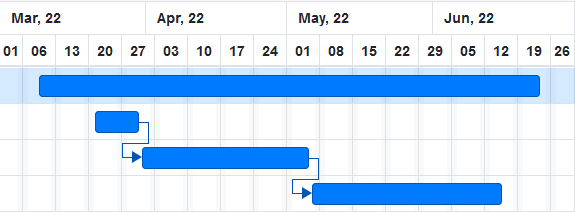
\includegraphics[width=\linewidth]{imagenes/digrama-gantt.png}
    \caption{Diagrama de Gantt. Gráfico.}
    \label{fig:figure2}
\end{figure}

Este gráfico corresponde con la duración de cada etapa, comenzando con la documentación. También se indica que hay etapas que para que estas se puedan empezar a desarrollar necesitan que la anterior este terminada, es el caso de la etapa de \textit{Desarrollo de la aplicación} y de \textit{Explotación de una vulnerabilidad}.

% Cada etapa se divide en una serie de tareas independientes que se deben de cumplir para poder completar una etapa.

% \subsubsection{Etapa 1}

% Las tareas a realizar para esta etapa son:

% \begin{itemize}
%     \item \textbf{Requisitos de elección del framework}
%     \item \textbf{Búsqueda de distintos frameworks}
%     \item \textbf{Análisis de los distintos entornos}
%     \item \textbf{Elección de un framework}
% \end{itemize}

%\section{Planificación a posteriori}